% Options for packages loaded elsewhere
\PassOptionsToPackage{unicode}{hyperref}
\PassOptionsToPackage{hyphens}{url}
%
\documentclass[
  12pt,
]{article}
\usepackage{amsmath,amssymb}
\usepackage{lmodern}
\usepackage{iftex}
\ifPDFTeX
  \usepackage[T1]{fontenc}
  \usepackage[utf8]{inputenc}
  \usepackage{textcomp} % provide euro and other symbols
\else % if luatex or xetex
  \usepackage{unicode-math}
  \defaultfontfeatures{Scale=MatchLowercase}
  \defaultfontfeatures[\rmfamily]{Ligatures=TeX,Scale=1}
\fi
% Use upquote if available, for straight quotes in verbatim environments
\IfFileExists{upquote.sty}{\usepackage{upquote}}{}
\IfFileExists{microtype.sty}{% use microtype if available
  \usepackage[]{microtype}
  \UseMicrotypeSet[protrusion]{basicmath} % disable protrusion for tt fonts
}{}
\makeatletter
\@ifundefined{KOMAClassName}{% if non-KOMA class
  \IfFileExists{parskip.sty}{%
    \usepackage{parskip}
  }{% else
    \setlength{\parindent}{0pt}
    \setlength{\parskip}{6pt plus 2pt minus 1pt}}
}{% if KOMA class
  \KOMAoptions{parskip=half}}
\makeatother
\usepackage{xcolor}
\usepackage[margin=1in]{geometry}
\usepackage{color}
\usepackage{fancyvrb}
\newcommand{\VerbBar}{|}
\newcommand{\VERB}{\Verb[commandchars=\\\{\}]}
\DefineVerbatimEnvironment{Highlighting}{Verbatim}{commandchars=\\\{\}}
% Add ',fontsize=\small' for more characters per line
\usepackage{framed}
\definecolor{shadecolor}{RGB}{248,248,248}
\newenvironment{Shaded}{\begin{snugshade}}{\end{snugshade}}
\newcommand{\AlertTok}[1]{\textcolor[rgb]{0.94,0.16,0.16}{#1}}
\newcommand{\AnnotationTok}[1]{\textcolor[rgb]{0.56,0.35,0.01}{\textbf{\textit{#1}}}}
\newcommand{\AttributeTok}[1]{\textcolor[rgb]{0.77,0.63,0.00}{#1}}
\newcommand{\BaseNTok}[1]{\textcolor[rgb]{0.00,0.00,0.81}{#1}}
\newcommand{\BuiltInTok}[1]{#1}
\newcommand{\CharTok}[1]{\textcolor[rgb]{0.31,0.60,0.02}{#1}}
\newcommand{\CommentTok}[1]{\textcolor[rgb]{0.56,0.35,0.01}{\textit{#1}}}
\newcommand{\CommentVarTok}[1]{\textcolor[rgb]{0.56,0.35,0.01}{\textbf{\textit{#1}}}}
\newcommand{\ConstantTok}[1]{\textcolor[rgb]{0.00,0.00,0.00}{#1}}
\newcommand{\ControlFlowTok}[1]{\textcolor[rgb]{0.13,0.29,0.53}{\textbf{#1}}}
\newcommand{\DataTypeTok}[1]{\textcolor[rgb]{0.13,0.29,0.53}{#1}}
\newcommand{\DecValTok}[1]{\textcolor[rgb]{0.00,0.00,0.81}{#1}}
\newcommand{\DocumentationTok}[1]{\textcolor[rgb]{0.56,0.35,0.01}{\textbf{\textit{#1}}}}
\newcommand{\ErrorTok}[1]{\textcolor[rgb]{0.64,0.00,0.00}{\textbf{#1}}}
\newcommand{\ExtensionTok}[1]{#1}
\newcommand{\FloatTok}[1]{\textcolor[rgb]{0.00,0.00,0.81}{#1}}
\newcommand{\FunctionTok}[1]{\textcolor[rgb]{0.00,0.00,0.00}{#1}}
\newcommand{\ImportTok}[1]{#1}
\newcommand{\InformationTok}[1]{\textcolor[rgb]{0.56,0.35,0.01}{\textbf{\textit{#1}}}}
\newcommand{\KeywordTok}[1]{\textcolor[rgb]{0.13,0.29,0.53}{\textbf{#1}}}
\newcommand{\NormalTok}[1]{#1}
\newcommand{\OperatorTok}[1]{\textcolor[rgb]{0.81,0.36,0.00}{\textbf{#1}}}
\newcommand{\OtherTok}[1]{\textcolor[rgb]{0.56,0.35,0.01}{#1}}
\newcommand{\PreprocessorTok}[1]{\textcolor[rgb]{0.56,0.35,0.01}{\textit{#1}}}
\newcommand{\RegionMarkerTok}[1]{#1}
\newcommand{\SpecialCharTok}[1]{\textcolor[rgb]{0.00,0.00,0.00}{#1}}
\newcommand{\SpecialStringTok}[1]{\textcolor[rgb]{0.31,0.60,0.02}{#1}}
\newcommand{\StringTok}[1]{\textcolor[rgb]{0.31,0.60,0.02}{#1}}
\newcommand{\VariableTok}[1]{\textcolor[rgb]{0.00,0.00,0.00}{#1}}
\newcommand{\VerbatimStringTok}[1]{\textcolor[rgb]{0.31,0.60,0.02}{#1}}
\newcommand{\WarningTok}[1]{\textcolor[rgb]{0.56,0.35,0.01}{\textbf{\textit{#1}}}}
\usepackage{graphicx}
\makeatletter
\def\maxwidth{\ifdim\Gin@nat@width>\linewidth\linewidth\else\Gin@nat@width\fi}
\def\maxheight{\ifdim\Gin@nat@height>\textheight\textheight\else\Gin@nat@height\fi}
\makeatother
% Scale images if necessary, so that they will not overflow the page
% margins by default, and it is still possible to overwrite the defaults
% using explicit options in \includegraphics[width, height, ...]{}
\setkeys{Gin}{width=\maxwidth,height=\maxheight,keepaspectratio}
% Set default figure placement to htbp
\makeatletter
\def\fps@figure{htbp}
\makeatother
\setlength{\emergencystretch}{3em} % prevent overfull lines
\providecommand{\tightlist}{%
  \setlength{\itemsep}{0pt}\setlength{\parskip}{0pt}}
\setcounter{secnumdepth}{-\maxdimen} % remove section numbering
\usepackage{xcolor}
\usepackage{hyperref}
\usepackage{pdfcomment}
\usepackage{fancyhdr} \pagestyle{fancy} \setlength{\headheight}{75pt} \setlength{\textheight}{600pt} \fancyhead[C]{} \fancyhead[L]{
\includegraphics{X:/DSA/shiny-uploads/images/PST_Equity_Edition-Trend_header.png}} \fancyhead[R]{} \fancyfoot[L]{\scriptsize{1011 Western Ave, Suite 500, Seattle WA 98104} \textcolor[HTML]{F05A28}. 206.464.7532 \textcolor[HTML]{F05A28}. www.psrc.org \textcolor[HTML]{F05A28}. November 2022} \fancyfoot[R]{\textcolor[HTML]{F05A28}\thepage} \fancyfoot[C]{} \renewcommand{\headrulewidth}{0pt} \renewcommand{\footrulewidth}{4pt} \renewcommand{\footrule}{\hbox to \headwidth{\color[HTML]{BCBEC0}\leaders\hrule height \footrulewidth\hfill}}
\usepackage{fontspec}
\ifLuaTeX
  \usepackage{selnolig}  % disable illegal ligatures
\fi
\IfFileExists{bookmark.sty}{\usepackage{bookmark}}{\usepackage{hyperref}}
\IfFileExists{xurl.sty}{\usepackage{xurl}}{} % add URL line breaks if available
\urlstyle{same} % disable monospaced font for URLs
\hypersetup{
  hidelinks,
  pdfcreator={LaTeX via pandoc}}

\author{}
\date{\vspace{-2.5em}}

\begin{document}

\setmainfont{Poppins}

\begin{verbatim}
## Warning: package 'dplyr' was built under R version 4.2.2
\end{verbatim}

\begin{verbatim}
## 
## Attaching package: 'dplyr'
\end{verbatim}

\begin{verbatim}
## The following objects are masked from 'package:stats':
## 
##     filter, lag
\end{verbatim}

\begin{verbatim}
## The following objects are masked from 'package:base':
## 
##     intersect, setdiff, setequal, union
\end{verbatim}

\begin{verbatim}
## Warning: package 'stringr' was built under R version 4.2.2
\end{verbatim}

\begin{verbatim}
## Warning: package 'ggplot2' was built under R version 4.2.2
\end{verbatim}

\begin{verbatim}
## Warning: package 'forcats' was built under R version 4.2.1
\end{verbatim}

\begin{verbatim}
## Warning: package 'odbc' was built under R version 4.2.1
\end{verbatim}

\begin{verbatim}
## Warning: package 'DBI' was built under R version 4.2.1
\end{verbatim}

\begin{verbatim}
## Warning: package 'tidyr' was built under R version 4.2.2
\end{verbatim}

\begin{verbatim}
## Warning: package 'srvyr' was built under R version 4.2.1
\end{verbatim}

\begin{verbatim}
## 
## Attaching package: 'srvyr'
\end{verbatim}

\begin{verbatim}
## The following object is masked from 'package:stats':
## 
##     filter
\end{verbatim}

\begin{verbatim}
## Loading required package: grid
\end{verbatim}

\begin{verbatim}
## Loading required package: Matrix
\end{verbatim}

\begin{verbatim}
## Warning: package 'Matrix' was built under R version 4.2.1
\end{verbatim}

\begin{verbatim}
## 
## Attaching package: 'Matrix'
\end{verbatim}

\begin{verbatim}
## The following objects are masked from 'package:tidyr':
## 
##     expand, pack, unpack
\end{verbatim}

\begin{verbatim}
## Loading required package: survival
\end{verbatim}

\begin{verbatim}
## 
## Attaching package: 'survey'
\end{verbatim}

\begin{verbatim}
## The following object is masked from 'package:graphics':
## 
##     dotchart
\end{verbatim}

\begin{verbatim}
## 
## Attaching package: 'psrccensus'
\end{verbatim}

\begin{verbatim}
## The following object is masked from 'package:psrc.travelsurvey':
## 
##     z_score
\end{verbatim}

\begin{verbatim}
## Warning: package 'tidyverse' was built under R version 4.2.1
\end{verbatim}

\begin{verbatim}
## -- Attaching packages --------------------------------------- tidyverse 1.3.2
## --
\end{verbatim}

\begin{verbatim}
## v tibble 3.1.8     v purrr  1.0.1
## v readr  2.1.3
\end{verbatim}

\begin{verbatim}
## Warning: package 'tibble' was built under R version 4.2.1
\end{verbatim}

\begin{verbatim}
## Warning: package 'readr' was built under R version 4.2.1
\end{verbatim}

\begin{verbatim}
## Warning: package 'purrr' was built under R version 4.2.2
\end{verbatim}

\begin{verbatim}
## -- Conflicts ------------------------------------------ tidyverse_conflicts() --
## x Matrix::expand() masks tidyr::expand()
## x srvyr::filter()  masks dplyr::filter(), stats::filter()
## x dplyr::lag()     masks stats::lag()
## x Matrix::pack()   masks tidyr::pack()
## x Matrix::unpack() masks tidyr::unpack()
\end{verbatim}

\begin{verbatim}
## Warning: package 'knitr' was built under R version 4.2.2
\end{verbatim}

\begin{verbatim}
## Linking to ImageMagick 6.9.12.3
## Enabled features: cairo, freetype, fftw, ghostscript, heic, lcms, pango, raw, rsvg, webp
## Disabled features: fontconfig, x11
\end{verbatim}

\begin{verbatim}
## Warning: package 'openxlsx' was built under R version 4.2.1
\end{verbatim}

\begin{verbatim}
## Warning: package 'htmlwidgets' was built under R version 4.2.2
\end{verbatim}

Megan's datapoints: Employment by age group 2019 Women tend to not be
employed, but do more caring travel

\begin{Shaded}
\begin{Highlighting}[]
\CommentTok{\# DATA ANALYSIS}
\CommentTok{\# read in hh survey trip data}
\NormalTok{db.connect }\OtherTok{\textless{}{-}} \ControlFlowTok{function}\NormalTok{(adatabase) \{}
\NormalTok{  elmer\_connection }\OtherTok{\textless{}{-}} \FunctionTok{dbConnect}\NormalTok{(}\FunctionTok{odbc}\NormalTok{(),}
                                \AttributeTok{driver =} \StringTok{"SQL Server"}\NormalTok{,}
                                \AttributeTok{server =} \StringTok{"AWS{-}PROD{-}SQL}\SpecialCharTok{\textbackslash{}\textbackslash{}}\StringTok{SOCKEYE"}\NormalTok{,}
                                \AttributeTok{database =}\NormalTok{ adatabase,}
                                \AttributeTok{trusted\_connection =} \StringTok{"yes"}
\NormalTok{  )}
\NormalTok{\}}

\CommentTok{\# read table}
\NormalTok{read.dt }\OtherTok{\textless{}{-}} \ControlFlowTok{function}\NormalTok{(adatabase, atable) \{}
\NormalTok{  elmer\_connection }\OtherTok{\textless{}{-}} \FunctionTok{db.connect}\NormalTok{(adatabase)}
\NormalTok{  dtelm }\OtherTok{\textless{}{-}} \FunctionTok{dbReadTable}\NormalTok{(elmer\_connection, }\FunctionTok{SQL}\NormalTok{(atable))}
  \FunctionTok{dbDisconnect}\NormalTok{(elmer\_connection)}
  \FunctionTok{return}\NormalTok{(dtelm)}
\NormalTok{\}}

\CommentTok{\# read{-}in variable metadata table for levels}
\NormalTok{vars\_meta }\OtherTok{\textless{}{-}} \FunctionTok{read.dt}\NormalTok{(}\StringTok{\textquotesingle{}Elmer\textquotesingle{}}\NormalTok{, }\StringTok{\textquotesingle{}HHSurvey.variable\_metadata\textquotesingle{}}\NormalTok{)}


\NormalTok{mode\_vars}\OtherTok{\textless{}{-}}\FunctionTok{c}\NormalTok{(}\StringTok{\textquotesingle{}mode\_1\textquotesingle{}}\NormalTok{, }\StringTok{\textquotesingle{}mode\_simple\textquotesingle{}}\NormalTok{, }\StringTok{\textquotesingle{}travelers\_total\textquotesingle{}}\NormalTok{)}
\NormalTok{other\_vars}\OtherTok{\textless{}{-}}\FunctionTok{c}\NormalTok{(}\StringTok{\textquotesingle{}final\_home\_rgcnum\textquotesingle{}}\NormalTok{, }\StringTok{\textquotesingle{}hhsize\textquotesingle{}}\NormalTok{, }\StringTok{\textquotesingle{}vehicle\_count\textquotesingle{}}\NormalTok{,  }\StringTok{"hhincome\_broad"}\NormalTok{, }\StringTok{\textquotesingle{}rent\_own\textquotesingle{}}\NormalTok{, }\StringTok{\textquotesingle{}res\_dur\textquotesingle{}}\NormalTok{, }\StringTok{\textquotesingle{}student\textquotesingle{}}\NormalTok{, }\StringTok{\textquotesingle{}education\textquotesingle{}}\NormalTok{,  }\StringTok{\textquotesingle{}hhincome\_detailed\textquotesingle{}}\NormalTok{, }\StringTok{"age"}\NormalTok{, }\StringTok{"age\_category"}\NormalTok{, }\StringTok{\textquotesingle{}race\_category\textquotesingle{}}\NormalTok{, }\StringTok{\textquotesingle{}race\_eth\_broad\textquotesingle{}}\NormalTok{, }\StringTok{\textquotesingle{}gender\textquotesingle{}}\NormalTok{, }\StringTok{\textquotesingle{}employment\textquotesingle{}}\NormalTok{,  }\StringTok{\textquotesingle{}lifecycle\textquotesingle{}}\NormalTok{, }\StringTok{\textquotesingle{}mode\_acc\textquotesingle{}}\NormalTok{, }\StringTok{\textquotesingle{}dest\_purpose\_cat\textquotesingle{}}\NormalTok{, }\StringTok{\textquotesingle{}origin\_purpose\_cat\textquotesingle{}}\NormalTok{, }\StringTok{\textquotesingle{}final\_home\_is\_rgc\textquotesingle{}}\NormalTok{)}
\NormalTok{trip\_path\_dist}\OtherTok{\textless{}{-}}\StringTok{\textquotesingle{}trip\_path\_distance\textquotesingle{}}
\NormalTok{all\_vars}\OtherTok{\textless{}{-}}\FunctionTok{c}\NormalTok{(mode\_vars, other\_vars, trip\_path\_dist)}

\NormalTok{data\_17\_19}\OtherTok{\textless{}{-}} \FunctionTok{get\_hhts}\NormalTok{(}\StringTok{"2017\_2019"}\NormalTok{, }\StringTok{"t"}\NormalTok{, }\AttributeTok{vars=}\NormalTok{all\_vars)}\SpecialCharTok{\%\textgreater{}\%} \FunctionTok{mutate}\NormalTok{(}\AttributeTok{year=}\FunctionTok{ifelse}\NormalTok{(survey}\SpecialCharTok{==}\StringTok{\textquotesingle{}2017\_2019\textquotesingle{}}\NormalTok{, }\StringTok{\textquotesingle{}2017/2019\textquotesingle{}}\NormalTok{, }\StringTok{\textquotesingle{}2021\textquotesingle{}}\NormalTok{))}

\NormalTok{data\_21}\OtherTok{\textless{}{-}} \FunctionTok{get\_hhts}\NormalTok{(}\StringTok{"2021"}\NormalTok{, }\StringTok{"t"}\NormalTok{, }\AttributeTok{vars=}\NormalTok{all\_vars)}\SpecialCharTok{\%\textgreater{}\%} \FunctionTok{mutate}\NormalTok{(}\AttributeTok{year=}\FunctionTok{ifelse}\NormalTok{(survey}\SpecialCharTok{==}\StringTok{\textquotesingle{}2017\_2019\textquotesingle{}}\NormalTok{, }\StringTok{\textquotesingle{}2017/2019\textquotesingle{}}\NormalTok{, }\StringTok{\textquotesingle{}2021\textquotesingle{}}\NormalTok{))}
\end{Highlighting}
\end{Shaded}

\begin{Shaded}
\begin{Highlighting}[]
\CommentTok{\# set up trip data for analysis}
\NormalTok{data\_17\_19}\OtherTok{\textless{}{-}}\NormalTok{data\_17\_19}\SpecialCharTok{\%\textgreater{}\%}\FunctionTok{mutate}\NormalTok{(}\AttributeTok{NoVehicles=}\FunctionTok{ifelse}\NormalTok{(vehicle\_count}\SpecialCharTok{==}\StringTok{\textquotesingle{}0 (no vehicles)\textquotesingle{}}\NormalTok{, }\StringTok{\textquotesingle{}No Vehicles\textquotesingle{}}\NormalTok{, }\StringTok{"Has Vehicles"}\NormalTok{))}\SpecialCharTok{\%\textgreater{}\%}
  \FunctionTok{mutate}\NormalTok{(}\AttributeTok{hhsize\_simple=}\FunctionTok{case\_when}\NormalTok{(hhsize}\SpecialCharTok{==} \StringTok{\textquotesingle{}4 people\textquotesingle{}} \SpecialCharTok{\textasciitilde{}}\StringTok{\textquotesingle{}4 or more people\textquotesingle{}}\NormalTok{,                                                                     hhsize}\SpecialCharTok{==} \StringTok{\textquotesingle{}5 people\textquotesingle{}} \SpecialCharTok{\textasciitilde{}}\StringTok{\textquotesingle{}4 or more people\textquotesingle{}}\NormalTok{,}
\NormalTok{                                 hhsize}\SpecialCharTok{==} \StringTok{\textquotesingle{}6 people\textquotesingle{}} \SpecialCharTok{\textasciitilde{}}\StringTok{\textquotesingle{}4 or more people\textquotesingle{}}\NormalTok{,}
\NormalTok{                                 hhsize}\SpecialCharTok{==} \StringTok{\textquotesingle{}7 people\textquotesingle{}} \SpecialCharTok{\textasciitilde{}}\StringTok{\textquotesingle{}4 or more people\textquotesingle{}}\NormalTok{,}
\NormalTok{                                 hhsize}\SpecialCharTok{==} \StringTok{\textquotesingle{}8 people\textquotesingle{}} \SpecialCharTok{\textasciitilde{}}\StringTok{\textquotesingle{}4 or more people\textquotesingle{}}\NormalTok{,}
\NormalTok{                                 hhsize}\SpecialCharTok{==} \StringTok{\textquotesingle{}12 people\textquotesingle{}} \SpecialCharTok{\textasciitilde{}}\StringTok{\textquotesingle{}4 or more people\textquotesingle{}}\NormalTok{,}
                                 \ConstantTok{TRUE} \SpecialCharTok{\textasciitilde{}}\NormalTok{ hhsize))}\SpecialCharTok{\%\textgreater{}\%}
  \FunctionTok{mutate}\NormalTok{(}\AttributeTok{hhincome\_100=} \FunctionTok{case\_when}\NormalTok{(hhincome\_broad}\SpecialCharTok{==}\StringTok{\textquotesingle{}$100,000{-}$199,000\textquotesingle{}} \SpecialCharTok{\textasciitilde{}} \StringTok{\textquotesingle{}$100,000 or more\textquotesingle{}}\NormalTok{,}
\NormalTok{                                 hhincome\_broad}\SpecialCharTok{==}\StringTok{\textquotesingle{}$200,000 or more\textquotesingle{}} \SpecialCharTok{\textasciitilde{}} \StringTok{\textquotesingle{}$100,000 or more\textquotesingle{}}\NormalTok{,}
                                 \ConstantTok{TRUE}\SpecialCharTok{\textasciitilde{}}\NormalTok{hhincome\_broad))}\SpecialCharTok{\%\textgreater{}\%}
  \FunctionTok{mutate}\NormalTok{(}\AttributeTok{edu\_simple=} \FunctionTok{case\_when}\NormalTok{(education}\SpecialCharTok{==}\StringTok{\textquotesingle{}Bachelor degree\textquotesingle{}} \SpecialCharTok{\textasciitilde{}} \StringTok{\textquotesingle{}Bachelors or higher\textquotesingle{}}\NormalTok{, }
\NormalTok{                               education}\SpecialCharTok{==}\StringTok{\textquotesingle{}Graduate/Post{-}graduate degree\textquotesingle{}} \SpecialCharTok{\textasciitilde{}} \StringTok{\textquotesingle{}Bachelors or higher\textquotesingle{}}\NormalTok{,}
                               \ConstantTok{TRUE} \SpecialCharTok{\textasciitilde{}} \StringTok{\textquotesingle{}Less than Bachelors degree\textquotesingle{}}\NormalTok{))}\SpecialCharTok{\%\textgreater{}\%}
  \FunctionTok{mutate}\NormalTok{(}\AttributeTok{age\_grp=} \FunctionTok{case\_when}\NormalTok{(age}\SpecialCharTok{==}\StringTok{\textquotesingle{}75{-}84 years\textquotesingle{}} \SpecialCharTok{\textasciitilde{}} \StringTok{\textquotesingle{}75 years or older\textquotesingle{}}\NormalTok{, }
\NormalTok{                            age }\SpecialCharTok{==} \StringTok{\textquotesingle{}85 or years older\textquotesingle{}} \SpecialCharTok{\textasciitilde{}} \StringTok{\textquotesingle{}75 years or older\textquotesingle{}}\NormalTok{,}
                            \ConstantTok{TRUE} \SpecialCharTok{\textasciitilde{}}\NormalTok{ age))}\SpecialCharTok{\%\textgreater{}\%}
  \FunctionTok{mutate}\NormalTok{(}\AttributeTok{gender\_grp=} \FunctionTok{case\_when}\NormalTok{(gender }\SpecialCharTok{==} \StringTok{\textquotesingle{}Prefer not to answer\textquotesingle{}} \SpecialCharTok{\textasciitilde{}} \StringTok{\textquotesingle{}Non{-}binary, another, prefer not to answer\textquotesingle{}}\NormalTok{,}
\NormalTok{                               gender}\SpecialCharTok{==}\StringTok{\textquotesingle{}Not listed here / prefer not to answer\textquotesingle{}} \SpecialCharTok{\textasciitilde{}} \StringTok{\textquotesingle{}Non{-}binary, another, prefer not to answer\textquotesingle{}}\NormalTok{,}
\NormalTok{                               gender}\SpecialCharTok{==}\StringTok{\textquotesingle{}Non{-}Binary\textquotesingle{}}\SpecialCharTok{\textasciitilde{}} \StringTok{\textquotesingle{}Non{-}binary, another, prefer not to answer\textquotesingle{}}\NormalTok{,}
\NormalTok{                               gender}\SpecialCharTok{==}\StringTok{\textquotesingle{}Another\textquotesingle{}}\SpecialCharTok{\textasciitilde{}} \StringTok{\textquotesingle{}Non{-}binary, another, prefer not to answer\textquotesingle{}}\NormalTok{,}
                               \ConstantTok{TRUE} \SpecialCharTok{\textasciitilde{}}\NormalTok{ gender))}\SpecialCharTok{\%\textgreater{}\%}\FunctionTok{mutate}\NormalTok{(}\AttributeTok{work\_purpose=}\FunctionTok{ifelse}\NormalTok{(dest\_purpose\_cat}\SpecialCharTok{==}\StringTok{\textquotesingle{}Work\textquotesingle{}}\NormalTok{, }\StringTok{\textquotesingle{}Work\textquotesingle{}}\NormalTok{, }\StringTok{\textquotesingle{}Not Work\textquotesingle{}}\NormalTok{))}\SpecialCharTok{\%\textgreater{}\%}
  
  \FunctionTok{mutate}\NormalTok{(}\AttributeTok{race\_short=} \FunctionTok{str\_extract}\NormalTok{(race\_eth\_broad,  }\StringTok{"\^{}[\^{} ]+"}\NormalTok{))}\SpecialCharTok{\%\textgreater{}\%}
  \FunctionTok{mutate}\NormalTok{(}\AttributeTok{simple\_purpose=}\FunctionTok{ifelse}\NormalTok{(dest\_purpose\_cat}\SpecialCharTok{==}\StringTok{\textquotesingle{}Home\textquotesingle{}}\NormalTok{, origin\_purpose\_cat, dest\_purpose\_cat))}\SpecialCharTok{\%\textgreater{}\%}
  \FunctionTok{mutate}\NormalTok{(}\AttributeTok{simple\_purpose=}\FunctionTok{case\_when}\NormalTok{(simple\_purpose}\SpecialCharTok{==}\StringTok{\textquotesingle{}Work\textquotesingle{}}\SpecialCharTok{\textasciitilde{}} \StringTok{\textquotesingle{}Work/School\textquotesingle{}}\NormalTok{,}
\NormalTok{                                  simple\_purpose}\SpecialCharTok{==}\StringTok{\textquotesingle{}School\textquotesingle{}}\SpecialCharTok{\textasciitilde{}} \StringTok{\textquotesingle{}Work/School\textquotesingle{}}\NormalTok{,}
\NormalTok{                                  simple\_purpose}\SpecialCharTok{==}\StringTok{\textquotesingle{}Work{-}related\textquotesingle{}}\SpecialCharTok{\textasciitilde{}} \StringTok{\textquotesingle{}Work/School\textquotesingle{}}\NormalTok{,}
\NormalTok{                                  simple\_purpose}\SpecialCharTok{==}\StringTok{\textquotesingle{}Shop\textquotesingle{}}\SpecialCharTok{\textasciitilde{}} \StringTok{\textquotesingle{}Shop\textquotesingle{}}\NormalTok{,}
\NormalTok{                                  simple\_purpose}\SpecialCharTok{==}\StringTok{\textquotesingle{}Escort\textquotesingle{}}\SpecialCharTok{\textasciitilde{}} \StringTok{\textquotesingle{}Escort Passenger\textquotesingle{}}\NormalTok{,}
\NormalTok{                                  simple\_purpose}\SpecialCharTok{==}\StringTok{\textquotesingle{}Errand/Other\textquotesingle{}}\SpecialCharTok{\textasciitilde{}} \StringTok{\textquotesingle{}Errands/Other\textquotesingle{}}\NormalTok{,}
\NormalTok{                                  simple\_purpose}\SpecialCharTok{==}\StringTok{\textquotesingle{}Change mode\textquotesingle{}}\SpecialCharTok{\textasciitilde{}} \StringTok{\textquotesingle{}Errands/Other\textquotesingle{}}\NormalTok{,}
\NormalTok{                                  simple\_purpose}\SpecialCharTok{==}\StringTok{\textquotesingle{}Social/Recreation\textquotesingle{}} \SpecialCharTok{\textasciitilde{}} \StringTok{\textquotesingle{}Social/Recreation/Meal\textquotesingle{}}\NormalTok{,}
\NormalTok{                                  simple\_purpose}\SpecialCharTok{==}\StringTok{\textquotesingle{}Meal\textquotesingle{}} \SpecialCharTok{\textasciitilde{}} \StringTok{\textquotesingle{}Social/Recreation/Meal\textquotesingle{}}\NormalTok{,}
\NormalTok{                                  simple\_purpose}\SpecialCharTok{==}\StringTok{\textquotesingle{}Home\textquotesingle{}} \SpecialCharTok{\textasciitilde{}}\StringTok{\textquotesingle{}Errands/Other\textquotesingle{}}\NormalTok{,}
                                  \FunctionTok{is.na}\NormalTok{(simple\_purpose) }\SpecialCharTok{\textasciitilde{}} \StringTok{\textquotesingle{}Errands/Other\textquotesingle{}}\NormalTok{,}
                                  \ConstantTok{TRUE} \SpecialCharTok{\textasciitilde{}}\NormalTok{ simple\_purpose))}\SpecialCharTok{\%\textgreater{}\%}\FunctionTok{mutate}\NormalTok{(}\AttributeTok{rgc=}\FunctionTok{as.factor}\NormalTok{(final\_home\_is\_rgc))}\SpecialCharTok{\%\textgreater{}\%}
  \FunctionTok{mutate}\NormalTok{(}\AttributeTok{non\_motorized\_mode=}\FunctionTok{ifelse}\NormalTok{((mode\_simple}\SpecialCharTok{==}\StringTok{\textquotesingle{}Walk\textquotesingle{}}\SpecialCharTok{|}\NormalTok{mode\_simple}\SpecialCharTok{==}\StringTok{\textquotesingle{}Bike\textquotesingle{}}\NormalTok{),}\StringTok{\textquotesingle{}Walk/Bike\textquotesingle{}}\NormalTok{, }\StringTok{\textquotesingle{}Not Walk/Bike\textquotesingle{}}\NormalTok{))}\SpecialCharTok{\%\textgreater{}\%}
  \FunctionTok{mutate}\NormalTok{(}\AttributeTok{mode\_acc\_walk=}\FunctionTok{ifelse}\NormalTok{(mode\_acc}\SpecialCharTok{==}\StringTok{\textquotesingle{}Walked or jogged\textquotesingle{}}\NormalTok{, }\StringTok{\textquotesingle{}Walked or jogged\textquotesingle{}}\NormalTok{, }\StringTok{\textquotesingle{}Other Access Mode\textquotesingle{}}\NormalTok{))}\SpecialCharTok{\%\textgreater{}\%}
  \FunctionTok{mutate}\NormalTok{(}\AttributeTok{travelers\_total\_grp=} \FunctionTok{case\_when}\NormalTok{(travelers\_total}\SpecialCharTok{\textless{}=}\DecValTok{1} \SpecialCharTok{\textasciitilde{}} \StringTok{\textquotesingle{}1\textquotesingle{}}\NormalTok{,}
\NormalTok{                                        travelers\_total}\SpecialCharTok{==}\DecValTok{2} \SpecialCharTok{\textasciitilde{}} \StringTok{\textquotesingle{}2\textquotesingle{}}\NormalTok{,}
\NormalTok{                                        travelers\_total}\SpecialCharTok{==}\DecValTok{3} \SpecialCharTok{\textasciitilde{}} \StringTok{\textquotesingle{}3+\textquotesingle{}}\NormalTok{,}
\NormalTok{                                        travelers\_total}\SpecialCharTok{==}\DecValTok{4} \SpecialCharTok{\textasciitilde{}} \StringTok{\textquotesingle{}4+\textquotesingle{}}\NormalTok{))}


\NormalTok{data\_21}\OtherTok{\textless{}{-}}\NormalTok{data\_21}\SpecialCharTok{\%\textgreater{}\%}\FunctionTok{mutate}\NormalTok{(}\AttributeTok{NoVehicles=}\FunctionTok{ifelse}\NormalTok{(vehicle\_count}\SpecialCharTok{==}\StringTok{\textquotesingle{}0 (no vehicles)\textquotesingle{}}\NormalTok{, }\StringTok{\textquotesingle{}No Vehicles\textquotesingle{}}\NormalTok{, }\StringTok{"Has Vehicles"}\NormalTok{))}\SpecialCharTok{\%\textgreater{}\%}
  \FunctionTok{mutate}\NormalTok{(}\AttributeTok{hhsize\_simple=}\FunctionTok{case\_when}\NormalTok{(hhsize}\SpecialCharTok{==} \StringTok{\textquotesingle{}4 people\textquotesingle{}} \SpecialCharTok{\textasciitilde{}}\StringTok{\textquotesingle{}4 or more people\textquotesingle{}}\NormalTok{,                                                                    hhsize}\SpecialCharTok{==} \StringTok{\textquotesingle{}5 people\textquotesingle{}} \SpecialCharTok{\textasciitilde{}}\StringTok{\textquotesingle{}4 or more people\textquotesingle{}}\NormalTok{,}
\NormalTok{                                 hhsize}\SpecialCharTok{==} \StringTok{\textquotesingle{}6 people\textquotesingle{}} \SpecialCharTok{\textasciitilde{}}\StringTok{\textquotesingle{}4 or more people\textquotesingle{}}\NormalTok{,}
\NormalTok{                                 hhsize}\SpecialCharTok{==} \StringTok{\textquotesingle{}7 people\textquotesingle{}} \SpecialCharTok{\textasciitilde{}}\StringTok{\textquotesingle{}4 or more people\textquotesingle{}}\NormalTok{,}
\NormalTok{                                 hhsize}\SpecialCharTok{==} \StringTok{\textquotesingle{}8 people\textquotesingle{}} \SpecialCharTok{\textasciitilde{}}\StringTok{\textquotesingle{}4 or more people\textquotesingle{}}\NormalTok{,}
\NormalTok{                                 hhsize}\SpecialCharTok{==} \StringTok{\textquotesingle{}12 people\textquotesingle{}} \SpecialCharTok{\textasciitilde{}}\StringTok{\textquotesingle{}4 or more people\textquotesingle{}}\NormalTok{,}
                                 \ConstantTok{TRUE} \SpecialCharTok{\textasciitilde{}}\NormalTok{ hhsize)) }\SpecialCharTok{\%\textgreater{}\%}
  \FunctionTok{mutate}\NormalTok{(}\AttributeTok{hhincome\_100=} \FunctionTok{case\_when}\NormalTok{(hhincome\_broad}\SpecialCharTok{==}\StringTok{\textquotesingle{}$100,000{-}$199,000\textquotesingle{}} \SpecialCharTok{\textasciitilde{}} \StringTok{\textquotesingle{}$100,000 or more\textquotesingle{}}\NormalTok{,}
\NormalTok{                                 hhincome\_broad}\SpecialCharTok{==}\StringTok{\textquotesingle{}$200,000 or more\textquotesingle{}} \SpecialCharTok{\textasciitilde{}} \StringTok{\textquotesingle{}$100,000 or more\textquotesingle{}}\NormalTok{,}
                                 \ConstantTok{TRUE}\SpecialCharTok{\textasciitilde{}}\NormalTok{hhincome\_broad))}\SpecialCharTok{\%\textgreater{}\%}
  \FunctionTok{mutate}\NormalTok{(}\AttributeTok{edu\_simple=} \FunctionTok{case\_when}\NormalTok{(education}\SpecialCharTok{==}\StringTok{\textquotesingle{}Bachelor degree\textquotesingle{}} \SpecialCharTok{\textasciitilde{}} \StringTok{\textquotesingle{}Bachelors or higher\textquotesingle{}}\NormalTok{, }
\NormalTok{                               education}\SpecialCharTok{==}\StringTok{\textquotesingle{}Graduate/Post{-}graduate degree\textquotesingle{}} \SpecialCharTok{\textasciitilde{}} \StringTok{\textquotesingle{}Bachelors or higher\textquotesingle{}}\NormalTok{,}
                               \ConstantTok{TRUE} \SpecialCharTok{\textasciitilde{}} \StringTok{\textquotesingle{}Less than Bachelors degree\textquotesingle{}}\NormalTok{))}\SpecialCharTok{\%\textgreater{}\%}
  \FunctionTok{mutate}\NormalTok{(}\AttributeTok{age\_grp=} \FunctionTok{case\_when}\NormalTok{(age}\SpecialCharTok{==}\StringTok{\textquotesingle{}75{-}84 years\textquotesingle{}} \SpecialCharTok{\textasciitilde{}} \StringTok{\textquotesingle{}75 years or older\textquotesingle{}}\NormalTok{, }
\NormalTok{                            age }\SpecialCharTok{==} \StringTok{\textquotesingle{}85 or years older\textquotesingle{}} \SpecialCharTok{\textasciitilde{}} \StringTok{\textquotesingle{}75 years or older\textquotesingle{}}\NormalTok{,}
                            \ConstantTok{TRUE} \SpecialCharTok{\textasciitilde{}}\NormalTok{ age))}\SpecialCharTok{\%\textgreater{}\%}
  \FunctionTok{mutate}\NormalTok{(}\AttributeTok{gender\_grp=} \FunctionTok{case\_when}\NormalTok{(gender }\SpecialCharTok{==} \StringTok{\textquotesingle{}Prefer not to answer\textquotesingle{}} \SpecialCharTok{\textasciitilde{}} \StringTok{\textquotesingle{}Non{-}binary, another, prefer not to answer\textquotesingle{}}\NormalTok{,}
\NormalTok{                               gender}\SpecialCharTok{==}\StringTok{\textquotesingle{}Not listed here / prefer not to answer\textquotesingle{}} \SpecialCharTok{\textasciitilde{}} \StringTok{\textquotesingle{}Non{-}binary, another, prefer not to answer\textquotesingle{}}\NormalTok{,}
\NormalTok{                               gender}\SpecialCharTok{==}\StringTok{\textquotesingle{}Non{-}Binary\textquotesingle{}}\SpecialCharTok{\textasciitilde{}} \StringTok{\textquotesingle{}Non{-}binary, another, prefer not to answer\textquotesingle{}}\NormalTok{, }
\NormalTok{                               gender}\SpecialCharTok{==}\StringTok{\textquotesingle{}Another\textquotesingle{}}\SpecialCharTok{\textasciitilde{}} \StringTok{\textquotesingle{}Non{-}binary, another, prefer not to answer\textquotesingle{}}\NormalTok{,}
                               \ConstantTok{TRUE} \SpecialCharTok{\textasciitilde{}}\NormalTok{ gender))}\SpecialCharTok{\%\textgreater{}\%}
  \FunctionTok{mutate}\NormalTok{(}\AttributeTok{work\_purpose=}\FunctionTok{ifelse}\NormalTok{(dest\_purpose\_cat}\SpecialCharTok{==}\StringTok{\textquotesingle{}Work\textquotesingle{}}\NormalTok{, }\StringTok{\textquotesingle{}Work\textquotesingle{}}\NormalTok{, }\StringTok{\textquotesingle{}Not Work\textquotesingle{}}\NormalTok{))}\SpecialCharTok{\%\textgreater{}\%}
  \FunctionTok{mutate}\NormalTok{(}\AttributeTok{simple\_purpose=}\FunctionTok{ifelse}\NormalTok{(dest\_purpose\_cat}\SpecialCharTok{==}\StringTok{\textquotesingle{}Home\textquotesingle{}}\NormalTok{, origin\_purpose\_cat, dest\_purpose\_cat))}\SpecialCharTok{\%\textgreater{}\%}
  \FunctionTok{mutate}\NormalTok{(}\AttributeTok{simple\_purpose=}\FunctionTok{case\_when}\NormalTok{(simple\_purpose}\SpecialCharTok{==}\StringTok{\textquotesingle{}Work\textquotesingle{}}\SpecialCharTok{\textasciitilde{}} \StringTok{\textquotesingle{}Work/School\textquotesingle{}}\NormalTok{,}
\NormalTok{                                  simple\_purpose}\SpecialCharTok{==}\StringTok{\textquotesingle{}School\textquotesingle{}}\SpecialCharTok{\textasciitilde{}} \StringTok{\textquotesingle{}Work/School\textquotesingle{}}\NormalTok{,}
\NormalTok{                                  simple\_purpose}\SpecialCharTok{==}\StringTok{\textquotesingle{}Work{-}related\textquotesingle{}}\SpecialCharTok{\textasciitilde{}} \StringTok{\textquotesingle{}Work/School\textquotesingle{}}\NormalTok{,}
\NormalTok{                                  simple\_purpose}\SpecialCharTok{==}\StringTok{\textquotesingle{}Shop\textquotesingle{}}\SpecialCharTok{\textasciitilde{}} \StringTok{\textquotesingle{}Shop\textquotesingle{}}\NormalTok{,}
\NormalTok{                                  simple\_purpose}\SpecialCharTok{==}\StringTok{\textquotesingle{}Escort\textquotesingle{}}\SpecialCharTok{\textasciitilde{}} \StringTok{\textquotesingle{}Escort Passenger\textquotesingle{}}\NormalTok{,}
\NormalTok{                                  simple\_purpose}\SpecialCharTok{==}\StringTok{\textquotesingle{}Errand/Other\textquotesingle{}}\SpecialCharTok{\textasciitilde{}} \StringTok{\textquotesingle{}Errands/Other\textquotesingle{}}\NormalTok{,}
\NormalTok{                                  simple\_purpose}\SpecialCharTok{==}\StringTok{\textquotesingle{}Change mode\textquotesingle{}}\SpecialCharTok{\textasciitilde{}} \StringTok{\textquotesingle{}Errands/Other\textquotesingle{}}\NormalTok{,}
\NormalTok{                                  simple\_purpose}\SpecialCharTok{==}\StringTok{\textquotesingle{}Social/Recreation\textquotesingle{}} \SpecialCharTok{\textasciitilde{}} \StringTok{\textquotesingle{}Social/Recreation/Meal\textquotesingle{}}\NormalTok{,}
\NormalTok{                                  simple\_purpose}\SpecialCharTok{==}\StringTok{\textquotesingle{}Meal\textquotesingle{}} \SpecialCharTok{\textasciitilde{}} \StringTok{\textquotesingle{}Social/Recreation/Meal\textquotesingle{}}\NormalTok{,}
\NormalTok{                                  simple\_purpose}\SpecialCharTok{==}\StringTok{\textquotesingle{}Home\textquotesingle{}} \SpecialCharTok{\textasciitilde{}}\StringTok{\textquotesingle{}Errands/Other\textquotesingle{}}\NormalTok{,}
                                  \FunctionTok{is.na}\NormalTok{(simple\_purpose) }\SpecialCharTok{\textasciitilde{}} \StringTok{\textquotesingle{}Errands/Other\textquotesingle{}}\NormalTok{,}
                                  \ConstantTok{TRUE} \SpecialCharTok{\textasciitilde{}}\NormalTok{ simple\_purpose))}\SpecialCharTok{\%\textgreater{}\%}\FunctionTok{mutate}\NormalTok{(}\AttributeTok{rgc=}\FunctionTok{as.factor}\NormalTok{(final\_home\_is\_rgc))}\SpecialCharTok{\%\textgreater{}\%}
  \FunctionTok{mutate}\NormalTok{(}\AttributeTok{non\_motorized\_mode=}\FunctionTok{ifelse}\NormalTok{((mode\_simple}\SpecialCharTok{==}\StringTok{\textquotesingle{}Walk\textquotesingle{}}\SpecialCharTok{|}\NormalTok{mode\_simple}\SpecialCharTok{==}\StringTok{\textquotesingle{}Bike\textquotesingle{}}\NormalTok{),}\StringTok{\textquotesingle{}Walk/Bike\textquotesingle{}}\NormalTok{, }\StringTok{\textquotesingle{}Not Walk/Bike\textquotesingle{}}\NormalTok{))}\SpecialCharTok{\%\textgreater{}\%}
  \FunctionTok{mutate}\NormalTok{(}\AttributeTok{mode\_acc\_walk=}\FunctionTok{ifelse}\NormalTok{(mode\_acc}\SpecialCharTok{==}\StringTok{\textquotesingle{}Walked or jogged\textquotesingle{}}\NormalTok{, }\StringTok{\textquotesingle{}Walked or jogged\textquotesingle{}}\NormalTok{, }\StringTok{\textquotesingle{}Other Access Mode\textquotesingle{}}\NormalTok{))}\SpecialCharTok{\%\textgreater{}\%}
  \FunctionTok{mutate}\NormalTok{(}\AttributeTok{travelers\_total\_grp=} \FunctionTok{case\_when}\NormalTok{(travelers\_total}\SpecialCharTok{\textless{}=}\DecValTok{1} \SpecialCharTok{\textasciitilde{}} \StringTok{\textquotesingle{}1\textquotesingle{}}\NormalTok{,}
\NormalTok{                                        travelers\_total}\SpecialCharTok{==}\DecValTok{2} \SpecialCharTok{\textasciitilde{}} \StringTok{\textquotesingle{}2\textquotesingle{}}\NormalTok{,}
\NormalTok{                                        travelers\_total}\SpecialCharTok{==}\DecValTok{3} \SpecialCharTok{\textasciitilde{}} \StringTok{\textquotesingle{}3+\textquotesingle{}}\NormalTok{,}
\NormalTok{                                        travelers\_total}\SpecialCharTok{==}\DecValTok{4} \SpecialCharTok{\textasciitilde{}} \StringTok{\textquotesingle{}4+\textquotesingle{}}\NormalTok{))}

\NormalTok{data\_17\_19}\SpecialCharTok{$}\NormalTok{hhincome\_100\_f}\OtherTok{=}\FunctionTok{factor}\NormalTok{(data\_17\_19}\SpecialCharTok{$}\NormalTok{hhincome\_100, }\AttributeTok{levels=}\FunctionTok{c}\NormalTok{(}\StringTok{"Prefer not to answer"}\NormalTok{,  }\StringTok{"$100,000 or more"}\NormalTok{,}\StringTok{"$75,000{-}$99,999"}\NormalTok{, }\StringTok{"$50,000{-}$74,999"}\NormalTok{ ,}\StringTok{"$25,000{-}$49,999"}\NormalTok{ , }\StringTok{"Under $25,000"}\NormalTok{  ))}

\NormalTok{data\_21}\SpecialCharTok{$}\NormalTok{hhincome\_100\_f}\OtherTok{=}\FunctionTok{factor}\NormalTok{(data\_21}\SpecialCharTok{$}\NormalTok{hhincome\_100, }\AttributeTok{levels=}\FunctionTok{c}\NormalTok{(}\StringTok{"Prefer not to answer"}\NormalTok{,  }\StringTok{"$100,000 or more"}\NormalTok{,}\StringTok{"$75,000{-}$99,999"}\NormalTok{, }\StringTok{"$50,000{-}$74,999"}\NormalTok{ ,}\StringTok{"$25,000{-}$49,999"}\NormalTok{ , }\StringTok{"Under $25,000"}\NormalTok{  ))}
\end{Highlighting}
\end{Shaded}

\begin{Shaded}
\begin{Highlighting}[]
\CommentTok{\# Trips by Purpose}
\CommentTok{\# Shows women do more caring trips; men more work and school; 2017/2019 has a stronger correlation with gender than 2021. COVID conditions?}

\NormalTok{  summs\_2017\_2019 }\OtherTok{\textless{}{-}} \FunctionTok{hhts\_count}\NormalTok{(data\_17\_19,}
                                        \AttributeTok{group\_vars=}\FunctionTok{c}\NormalTok{(}\StringTok{\textquotesingle{}gender\textquotesingle{}}\NormalTok{,}\StringTok{\textquotesingle{}simple\_purpose\textquotesingle{}}\NormalTok{),}
                                        \AttributeTok{spec\_wgt=}\StringTok{\textquotesingle{}trip\_adult\_weight\_2017\_2019\textquotesingle{}}\NormalTok{)}\SpecialCharTok{\%\textgreater{}\%}\FunctionTok{drop\_na}\NormalTok{(}\FunctionTok{c}\NormalTok{(}\StringTok{\textquotesingle{}gender\textquotesingle{}}\NormalTok{, }\StringTok{\textquotesingle{}simple\_purpose\textquotesingle{}}\NormalTok{))}\SpecialCharTok{\%\textgreater{}\%}\FunctionTok{filter}\NormalTok{(simple\_purpose}\SpecialCharTok{!=}\StringTok{\textquotesingle{}Total\textquotesingle{}}\NormalTok{)}\SpecialCharTok{\%\textgreater{}\%}\FunctionTok{filter}\NormalTok{(gender }\SpecialCharTok{\%in\%} \FunctionTok{c}\NormalTok{(}\StringTok{\textquotesingle{}Female\textquotesingle{}}\NormalTok{, }\StringTok{\textquotesingle{}Male\textquotesingle{}}\NormalTok{) )}

\NormalTok{  summs\_2021 }\OtherTok{\textless{}{-}} \FunctionTok{hhts\_count}\NormalTok{(data\_21,}
                                   \AttributeTok{group\_vars=}\FunctionTok{c}\NormalTok{(}\StringTok{\textquotesingle{}gender\textquotesingle{}}\NormalTok{,}\StringTok{\textquotesingle{}simple\_purpose\textquotesingle{}}\NormalTok{),}
                                   \AttributeTok{spec\_wgt=}\StringTok{\textquotesingle{}trip\_adult\_weight\_2021\textquotesingle{}}\NormalTok{) }\SpecialCharTok{\%\textgreater{}\%}\FunctionTok{drop\_na}\NormalTok{(}\FunctionTok{c}\NormalTok{(}\StringTok{\textquotesingle{}gender\textquotesingle{}}\NormalTok{, }\StringTok{\textquotesingle{}simple\_purpose\textquotesingle{}}\NormalTok{))}\SpecialCharTok{\%\textgreater{}\%}\FunctionTok{filter}\NormalTok{(simple\_purpose}\SpecialCharTok{!=}\StringTok{\textquotesingle{}Total\textquotesingle{}}\NormalTok{)}\SpecialCharTok{\%\textgreater{}\%}\FunctionTok{filter}\NormalTok{(gender }\SpecialCharTok{\%in\%} \FunctionTok{c}\NormalTok{(}\StringTok{\textquotesingle{}Female\textquotesingle{}}\NormalTok{, }\StringTok{\textquotesingle{}Male\textquotesingle{}}\NormalTok{) )}
  
 

\CommentTok{\#static\_column\_chart(t= summs\_2017\_2019, x=\textquotesingle{}simple\_purpose\textquotesingle{}, y=\textquotesingle{}share\textquotesingle{},  fill=\textquotesingle{}gender\textquotesingle{}, moe=\textquotesingle{}share\_moe\textquotesingle{}, est=\textquotesingle{}percent\textquotesingle{})}
\CommentTok{\#static\_column\_chart(t= summs\_2021, x=\textquotesingle{}simple\_purpose\textquotesingle{}, y=\textquotesingle{}share\textquotesingle{},  fill=\textquotesingle{}gender\textquotesingle{}, moe=\textquotesingle{}share\_moe\textquotesingle{}, est=\textquotesingle{}percent\textquotesingle{})}
\end{Highlighting}
\end{Shaded}

\begin{Shaded}
\begin{Highlighting}[]
\CommentTok{\# Trips by Number of Travelers}

\CommentTok{\# Women tend to travel with more people}

\NormalTok{data\_17\_19\_big\_hh}\OtherTok{\textless{}{-}}\NormalTok{ data\_17\_19}\SpecialCharTok{\%\textgreater{}\%}
  \FunctionTok{filter}\NormalTok{(}\SpecialCharTok{!}\NormalTok{hhsize }\SpecialCharTok{\%in\%} \FunctionTok{c}\NormalTok{(}\StringTok{\textquotesingle{}1 person\textquotesingle{}}\NormalTok{, }\StringTok{\textquotesingle{}2 people\textquotesingle{}}\NormalTok{))}
\NormalTok{data\_21\_big\_hh}\OtherTok{\textless{}{-}}\NormalTok{data\_21}\SpecialCharTok{\%\textgreater{}\%}
  \FunctionTok{filter}\NormalTok{(}\SpecialCharTok{!}\NormalTok{hhsize }\SpecialCharTok{\%in\%} \FunctionTok{c}\NormalTok{(}\StringTok{\textquotesingle{}1 person\textquotesingle{}}\NormalTok{, }\StringTok{\textquotesingle{}2 people\textquotesingle{}}\NormalTok{))}

\NormalTok{  summs\_2017\_2019 }\OtherTok{\textless{}{-}} \FunctionTok{hhts\_count}\NormalTok{(data\_17\_19\_big\_hh,}
                                        \AttributeTok{group\_vars=}\FunctionTok{c}\NormalTok{(}\StringTok{\textquotesingle{}gender\textquotesingle{}}\NormalTok{,}\StringTok{\textquotesingle{}travelers\_total\_grp\textquotesingle{}}\NormalTok{),}
                                        \AttributeTok{spec\_wgt=}\StringTok{\textquotesingle{}trip\_adult\_weight\_2017\_2019\textquotesingle{}}\NormalTok{)}\SpecialCharTok{\%\textgreater{}\%}\FunctionTok{drop\_na}\NormalTok{(}\FunctionTok{c}\NormalTok{(}\StringTok{\textquotesingle{}gender\textquotesingle{}}\NormalTok{, }\StringTok{\textquotesingle{}travelers\_total\_grp\textquotesingle{}}\NormalTok{))}\SpecialCharTok{\%\textgreater{}\%}\FunctionTok{filter}\NormalTok{(travelers\_total\_grp}\SpecialCharTok{!=}\StringTok{\textquotesingle{}Total\textquotesingle{}}\NormalTok{)}\SpecialCharTok{\%\textgreater{}\%}\FunctionTok{filter}\NormalTok{(travelers\_total\_grp}\SpecialCharTok{!=}\StringTok{\textquotesingle{}1\textquotesingle{}}\NormalTok{)}\SpecialCharTok{\%\textgreater{}\%}\FunctionTok{filter}\NormalTok{(gender }\SpecialCharTok{\%in\%} \FunctionTok{c}\NormalTok{(}\StringTok{\textquotesingle{}Female\textquotesingle{}}\NormalTok{, }\StringTok{\textquotesingle{}Male\textquotesingle{}}\NormalTok{) )}

\NormalTok{  summs\_2021 }\OtherTok{\textless{}{-}} \FunctionTok{hhts\_count}\NormalTok{(data\_21\_big\_hh,}
                                   \AttributeTok{group\_vars=}\FunctionTok{c}\NormalTok{(}\StringTok{\textquotesingle{}gender\textquotesingle{}}\NormalTok{,}\StringTok{\textquotesingle{}travelers\_total\_grp\textquotesingle{}}\NormalTok{),}
                                   \AttributeTok{spec\_wgt=}\StringTok{\textquotesingle{}trip\_adult\_weight\_2021\textquotesingle{}}\NormalTok{) }\SpecialCharTok{\%\textgreater{}\%}\FunctionTok{drop\_na}\NormalTok{(}\FunctionTok{c}\NormalTok{(}\StringTok{\textquotesingle{}gender\textquotesingle{}}\NormalTok{, }\StringTok{\textquotesingle{}travelers\_total\_grp\textquotesingle{}}\NormalTok{))}\SpecialCharTok{\%\textgreater{}\%}\FunctionTok{filter}\NormalTok{(travelers\_total\_grp}\SpecialCharTok{!=}\StringTok{\textquotesingle{}Total\textquotesingle{}}\NormalTok{)}\SpecialCharTok{\%\textgreater{}\%}\FunctionTok{filter}\NormalTok{(travelers\_total\_grp}\SpecialCharTok{!=}\StringTok{\textquotesingle{}1\textquotesingle{}}\NormalTok{)}\SpecialCharTok{\%\textgreater{}\%}\FunctionTok{filter}\NormalTok{(gender }\SpecialCharTok{\%in\%} \FunctionTok{c}\NormalTok{(}\StringTok{\textquotesingle{}Female\textquotesingle{}}\NormalTok{, }\StringTok{\textquotesingle{}Male\textquotesingle{}}\NormalTok{) )}
  
 

\FunctionTok{static\_column\_chart}\NormalTok{(}\AttributeTok{t=}\NormalTok{ summs\_2017\_2019, }\AttributeTok{x=}\StringTok{\textquotesingle{}travelers\_total\_grp\textquotesingle{}}\NormalTok{, }\AttributeTok{y=}\StringTok{\textquotesingle{}share\textquotesingle{}}\NormalTok{,  }\AttributeTok{fill=}\StringTok{\textquotesingle{}gender\textquotesingle{}}\NormalTok{, }\AttributeTok{moe=}\StringTok{\textquotesingle{}share\_moe\textquotesingle{}}\NormalTok{, }\AttributeTok{est=}\StringTok{\textquotesingle{}percent\textquotesingle{}}\NormalTok{)}
\end{Highlighting}
\end{Shaded}

\includegraphics{womens_history_files/figure-latex/unnamed-chunk-4-1.pdf}

\begin{Shaded}
\begin{Highlighting}[]
\FunctionTok{static\_column\_chart}\NormalTok{(}\AttributeTok{t=}\NormalTok{ summs\_2021, }\AttributeTok{x=}\StringTok{\textquotesingle{}travelers\_total\_grp\textquotesingle{}}\NormalTok{, }\AttributeTok{y=}\StringTok{\textquotesingle{}share\textquotesingle{}}\NormalTok{,  }\AttributeTok{fill=}\StringTok{\textquotesingle{}gender\textquotesingle{}}\NormalTok{, }\AttributeTok{moe=}\StringTok{\textquotesingle{}share\_moe\textquotesingle{}}\NormalTok{, }\AttributeTok{est=}\StringTok{\textquotesingle{}percent\textquotesingle{}}\NormalTok{)}
\end{Highlighting}
\end{Shaded}

\includegraphics{womens_history_files/figure-latex/unnamed-chunk-4-2.pdf}

\begin{Shaded}
\begin{Highlighting}[]
\NormalTok{  summs\_2017\_2019 }\OtherTok{\textless{}{-}} \FunctionTok{hhts\_count}\NormalTok{(data\_17\_19,}
                                        \AttributeTok{group\_vars=}\FunctionTok{c}\NormalTok{(}\StringTok{\textquotesingle{}gender\textquotesingle{}}\NormalTok{,}\StringTok{\textquotesingle{}mode\_simple\textquotesingle{}}\NormalTok{),}
                                        \AttributeTok{spec\_wgt=}\StringTok{\textquotesingle{}trip\_adult\_weight\_2017\_2019\textquotesingle{}}\NormalTok{)}\SpecialCharTok{\%\textgreater{}\%}\FunctionTok{drop\_na}\NormalTok{(}\FunctionTok{c}\NormalTok{(}\StringTok{\textquotesingle{}gender\textquotesingle{}}\NormalTok{, }\StringTok{\textquotesingle{}mode\_simple\textquotesingle{}}\NormalTok{))}\SpecialCharTok{\%\textgreater{}\%}\FunctionTok{filter}\NormalTok{(mode\_simple}\SpecialCharTok{==}\StringTok{\textquotesingle{}Bike\textquotesingle{}}\NormalTok{)}\SpecialCharTok{\%\textgreater{}\%}\FunctionTok{filter}\NormalTok{(gender }\SpecialCharTok{\%in\%} \FunctionTok{c}\NormalTok{(}\StringTok{\textquotesingle{}Female\textquotesingle{}}\NormalTok{, }\StringTok{\textquotesingle{}Male\textquotesingle{}}\NormalTok{) )}

\NormalTok{  summs\_2021 }\OtherTok{\textless{}{-}} \FunctionTok{hhts\_count}\NormalTok{(data\_21,}
                                   \AttributeTok{group\_vars=}\FunctionTok{c}\NormalTok{(}\StringTok{\textquotesingle{}gender\textquotesingle{}}\NormalTok{,}\StringTok{\textquotesingle{}mode\_simple\textquotesingle{}}\NormalTok{),}
                                   \AttributeTok{spec\_wgt=}\StringTok{\textquotesingle{}trip\_adult\_weight\_2021\textquotesingle{}}\NormalTok{) }\SpecialCharTok{\%\textgreater{}\%}\FunctionTok{drop\_na}\NormalTok{(}\FunctionTok{c}\NormalTok{(}\StringTok{\textquotesingle{}gender\textquotesingle{}}\NormalTok{, }\StringTok{\textquotesingle{}mode\_simple\textquotesingle{}}\NormalTok{))}\SpecialCharTok{\%\textgreater{}\%}\FunctionTok{filter}\NormalTok{(mode\_simple}\SpecialCharTok{==}\StringTok{\textquotesingle{}Bike\textquotesingle{}}\NormalTok{)}\SpecialCharTok{\%\textgreater{}\%}\FunctionTok{filter}\NormalTok{(gender }\SpecialCharTok{\%in\%} \FunctionTok{c}\NormalTok{(}\StringTok{\textquotesingle{}Female\textquotesingle{}}\NormalTok{, }\StringTok{\textquotesingle{}Male\textquotesingle{}}\NormalTok{) )}
  
 

\FunctionTok{static\_column\_chart}\NormalTok{(}\AttributeTok{t=}\NormalTok{ summs\_2017\_2019, }\AttributeTok{x=}\StringTok{\textquotesingle{}mode\_simple\textquotesingle{}}\NormalTok{, }\AttributeTok{y=}\StringTok{\textquotesingle{}count\textquotesingle{}}\NormalTok{,  }\AttributeTok{fill=}\StringTok{\textquotesingle{}gender\textquotesingle{}}\NormalTok{, }\AttributeTok{moe=}\StringTok{\textquotesingle{}count\_moe\textquotesingle{}}\NormalTok{, }\AttributeTok{est=}\StringTok{\textquotesingle{}number\textquotesingle{}}\NormalTok{)}
\end{Highlighting}
\end{Shaded}

\includegraphics{womens_history_files/figure-latex/unnamed-chunk-5-1.pdf}

\begin{Shaded}
\begin{Highlighting}[]
\FunctionTok{static\_column\_chart}\NormalTok{(}\AttributeTok{t=}\NormalTok{ summs\_2021, }\AttributeTok{x=}\StringTok{\textquotesingle{}mode\_simple\textquotesingle{}}\NormalTok{, }\AttributeTok{y=}\StringTok{\textquotesingle{}count\textquotesingle{}}\NormalTok{,  }\AttributeTok{fill=}\StringTok{\textquotesingle{}gender\textquotesingle{}}\NormalTok{, }\AttributeTok{moe=}\StringTok{\textquotesingle{}count\_moe\textquotesingle{}}\NormalTok{, }\AttributeTok{est=}\StringTok{\textquotesingle{}number\textquotesingle{}}\NormalTok{)}
\end{Highlighting}
\end{Shaded}

\includegraphics{womens_history_files/figure-latex/unnamed-chunk-5-2.pdf}
Post-COVID Looking forward Working at home Continued Aging Telecommute
rates What else?

Transit service needs to be more all day, not just to downtown

\hypertarget{celebrating-womens-history}{%
\section{Celebrating Women's History}\label{celebrating-womens-history}}

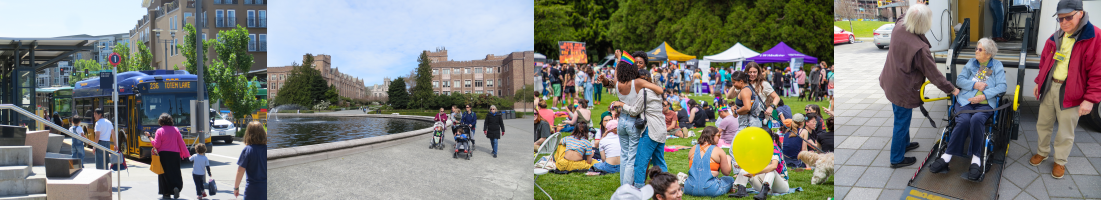
\includegraphics[width=1\textwidth,height=\textheight]{women_image_header.png}

Women represent a significant portion of the older population. Unique
needs.

Failing women's needs: Cycling network - results

\begin{flushleft}

notes: 
Fewer women work than men. Women take few work trips, more caregiving related trips, more household chore trips.The transit system was initially designed around traveling to a central city work location- which may not meet women's needs as well as men's (on average).Women live longer than men, so that at older ages there are many more women who have unique travel needs than men.Older people (who tend to be women more often) have more need for transit in off-peak hours and specialized transportation services.Women bike much less than men. Some of this is undoubtedly because of bike network design not being safe for all people.How can the transportation and land use system better accommodate older people, household maintenance and caregiving needs? Addressing these questions will improve the system for all genders.


Increase in telecommuting may be a double edged sword for women- still have hh responsibilities; but also juggling work



start with 2017/2019 data; transition to pandemic data?


according to 2021 hhts, 103, 000 women live in a household without a car; 86,000 men

from: http://libraryarchives.metro.net/DB_Attachments/2019-0294/UnderstandingHowWomenTravel_FullReport_FINAL.pdf

Travel Behavior Trends
Through the analysis in this report, key trends
emerge that differentiate women’s travel patterns
from men’s travel patterns, across all modes. » Across all modes, more women are making many
trips (7 or more) per day than men and more
women than men are not making any trips per day.
This means women may experience more exposure
to travel burdens (cost, stress, or safety risks), or
may be more likely to be isolated or disconnected
from the opportunities that travel affords.
» Women in Los Angeles also make shorter trips
than men, which is potentially driven by workforce
participation rates, location of employment
opportunities, and taking household-serving trips
that tend to be more localized.
» Women’s trips are more varied to a broader spread
of destinations, and are more likely to primarily
serve the needs of someone else.
» Women are more likely to live in a car-free or carlight household, take more trips with other people,
and take fewer single-occupant car trips than men.
» Women are also more likely to carpool or get a ride
from a family member or friend if they don’t have
a driver’s license.
These findings show that women may need to adjust
their own schedule and travel needs to accommodate
others, and in doing so, give up some of their own
autonomy and control over when and how they travel.
Despite these challenges and tradeoffs,
women show ingenuity in arranging their
schedules to meet their travel needs. » Women are more likely to trip-chain, or make
stops along the way to other destinations, and
describe consolidating all their errand trips into
one day where they will have access to a vehicle.
» Women in Los Angeles are also more likely than
men to travel mid-day, with a travel peak around 2
PM when transit service may be reduced.

Among female riders, almost 90% ride the system
more than three days per week.
» 57% of women bring their children on transit.
» Women ride transit because they do not have a
car, because they want to avoid traffic, or because
they do not have a license. Two of these three
reasons indicate that women who ride transit
do so because they have fewer
transportation options, and may
have less access to economic
opportunities as a result.
Still, many women do use transit
to access economic opportunity.
» Over 85% of women riders use
Metro to travel to work or school,
and of those women, 32% also use
Metro to run errands or complete
recreational trips.
Among people who make household
serving trips most frequently,
these trips comprise the same
share for women whether they use
transit or not; for men, the share of
household-serving trips declines if
they are transit users. This shows
that while men are more likely to
find alternatives to using transit to
complete household-serving trips
(using a different mode or taking
fewer trips), women are less likely
to find an alternative, and instead
work to make the transit system work for their needs.
Although the rate of adoption for TNCs like Uber and
Lyft is the same for men and women, women are more
likely than men to report that their transit use has
stayed the same as they have also begun to use TNCs.
» Women are more likely than men to say they use
TNCs for trips that transit does not serve, while
men are more likely to say they use TNCs to reach a
transit stop or station. The trips that are not served
by transit may be related to time or location, as
women’s needs differ from men’s needs by both
time of day and location.
These travel behavior findings point towards many
opportunities to adjust the services provided by Metro
to better meet the travel needs expressed by those
who are using transit. Development of a Gender Action
Plan - or a tactical plan to implement policy, design,
and service changes throughout the agency - would
help to articulate the immediate opportunities and
long-term goals that would create a system that
better serves women. Adjustments to services, vehicle
design, and policy would help minimize the time,
cost, safety, and physical burdens of riding transit
for the more than half of all riders who are women.
» The findings from Understanding
How Women Travel about women’s
mode choices, how likely they are to
travel with others in their care, and
their complex trip-chaining patterns
could all inform adjustments to
Metro’s fare policy to make it more
equitable towards women and more
cost-competitive with driving and
carpooling.
»Findings about women’s trip
purposes and primary responsibility
for household errands could all
inform the way transit vehicles,
transit stations, and bus stops are
designed, so that space for traveling
with others and carrying bags and
other belongings could be better
accommodated.
»Findings about when women are
traveling and average trip lengths
could inform new service offerings
that meet a mid-day peak travel
demand and provide better direct
connections over long distances while
minimizing transfers. 


Vehicle access issues disproportionately affect women. 

Financial access also disproportionately
affects women. Low-income women, in
particular, carry a disproportiona

\end{flushleft}

\hypertarget{some-header}{%
\subsection{some header}\label{some-header}}

\begin{flushleft}
more words
\end{flushleft}

\subsection{Conclusion}
\begin{flushleft}
someotherwords
\end{flushleft}

\fancyhead[L]{}

\end{document}
